\documentclass[tikz,border=10pt]{standalone}
\usepackage{tikz}
\usetikzlibrary{arrows.meta}

\begin{document}
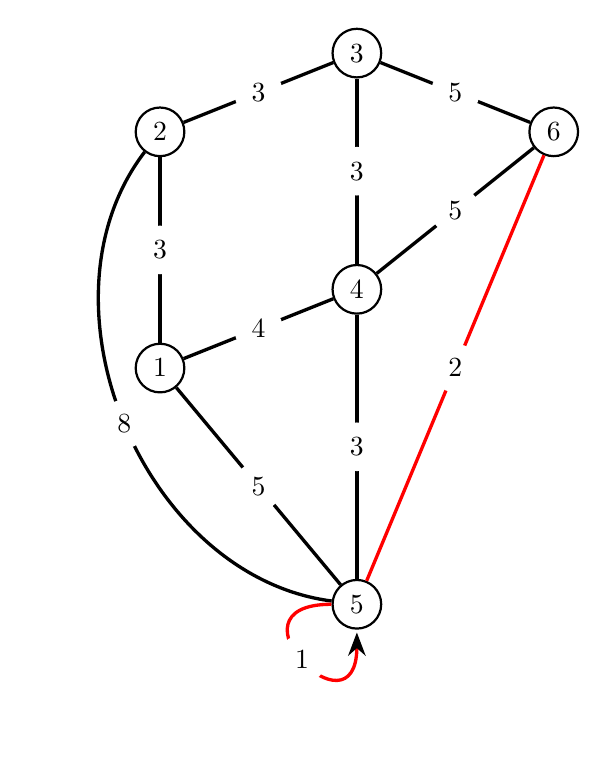
\begin{tikzpicture}
\begin{scope}[every node/.style={circle,thick,draw}]
    \node[draw=black] (1) at (0,0) {1};
    %\node[rectangle,draw=gray] (1cost) at (-0.5,0.5) {$0$};
    \node[draw=black] (2) at (0,3) {2};
    %\node[rectangle,draw=gray] (2cost) at (-0.6,3) {$3$};
    \node[draw=black] (3) at (2.5,4) {3};
    %\node[rectangle,draw=gray] (3cost) at (1.9,4.3) {$6$};
    \node[draw=black] (4) at (2.5,1) {4};
    %\node[rectangle,draw=gray] (4cost) at (1.9,1.3) {$4$};
    \node[draw=black] (5) at (2.5,-3) {5};
    %\node[rectangle,draw=gray] (5cost) at (3.0,-2.5) {$5$};
    \node[draw=black] (6) at (5,3) {6} ;
    %\node[rectangle,draw=gray] (6cost) at (5.5,3.5) {$7$};
\end{scope}

\begin{scope}[>={Stealth[black]},
              every node/.style={fill=white,circle},
              every edge/.style={draw=black,very thick}]
    \path [-] (1) edge[draw=black] node {$3$} (2);
    \path [-] (2) edge[draw=black] node {$3$} (3);
    \path [-] (1) edge[draw=black] node {$4$} (4);
    \path [-] (4) edge[draw=black] node {$3$} (3);
    \path [-] (1) edge[draw=black] node {$5$} (5);
    \path [-] (4) edge[draw=black] node {$3$} (5);
    \path [-] (4) edge[draw=black] node {$5$} (6);
    \path [-] (3) edge[draw=black] node {$5$} (6);
    \path [-] (5) edge[draw=red] node {$2$} (6); 
    \path [-] (2) edge[bend right=60, draw=black] node {$8$} (5); 
    \path [-] (5) edge[draw=red, out=180, in=-90, loop] node {$1$} (); 
\end{scope}
\end{tikzpicture}
\end{document}